\documentclass[12pt,a4paper,twoside]{scrreprt}
\usepackage[spanish]{babel}
\usepackage{fontspec}
\usepackage{parskip}
\usepackage{float}
\usepackage[
    font=normalsize,
    labelfont={bf},
    format=plain,
    justification=justified,
    singlelinecheck=false,
    indention=0pt
]{caption}
\usepackage[style=vancouver, backend=biber]{biblatex}
\usepackage{hyperref}
\usepackage{geometry}
\usepackage{graphicx}
\usepackage{setspace}
\usepackage{xcolor}
\usepackage{enumitem}
\usepackage{newunicodechar} 
\usepackage{longtable} 
\usepackage{array}           
\usepackage{ragged2e}        
\usepackage{booktabs}        
\usepackage{colortbl}            
\usepackage{appendix}
\usepackage{afterpage}
\usepackage{placeins} 
\usepackage{subcaption}
\usepackage{rotating} 

% Márgenes del documento
\geometry{left=3cm, right=2.5cm, top=2.5cm, bottom=2.5cm}
% Interlineado
\setstretch{1.5}
% Fuente
\setmainfont{Calibri}
% Color UNIR
\definecolor{UNIR}{HTML}{0098CD}
% Página en blanco
\newcommand{\blankpage}{
\newpage
\thispagestyle{empty}
\mbox{}
\newpage
}
% Formato UNIR...
\RedeclareSectionCommand[
  beforeskip=0pt,
  afterskip=20pt  
]{chapter}
% Posición del número de página
\setlength{\footskip}{35pt} 
% Epígrafes de apartados 
\newfontfamily\calibri{Calibri}
\newfontfamily\calibrilight{Calibri Light}
\setkomafont{disposition}{\normalfont}
\setkomafont{chapter}{\color{UNIR}\calibrilight\fontsize{18}{22}\selectfont}  
\renewcommand*{\chapterformat}{%
\thechapter.\enskip}
\setkomafont{section}{\color{UNIR}\calibrilight\fontsize{14}{17}\selectfont}
\setkomafont{subsection}{\bfseries\calibri\fontsize{12}{15}\selectfont}
\setkomafont{subsubsection}{\calibri\fontsize{12}{15}\selectfont}
\setcounter{secnumdepth}{3}
\RedeclareSectionCommand[
  beforeskip=8pt, % espacio antes del título de sección
  afterskip=8pt   % espacio después del título de sección
]{section}
\RedeclareSectionCommand[
  beforeskip=0pt,   % espacio antes del título del capítulo (puedes ajustar)
  afterskip=5pt     % espacio justo después del título del capítulo
]{chapter}
\RedeclareSectionCommand[
  beforeskip=8pt, % espacio antes del título de sección
  afterskip=8pt   % espacio después del título de sección
]{subsection}
\RedeclareSectionCommand[
  beforeskip=8pt, % espacio antes del título de subsubsección
  afterskip=8pt   % espacio después del título de subsubsección
]{subsubsection}

\captionsetup{labelfont=bf, textfont={normalsize,it}}

% 'Tabla' en lugar de 'cuadro'
\addto\captionsspanish{\renewcommand{\tablename}{Tabla}}
% ancho caption
\setlength{\LTcapwidth}{\textwidth} 

% Reducir espacio entre filas de las tablas
\renewcommand{\arraystretch}{0.6} 
\makeatletter
\patchcmd{\@arrayparboxrestore}
  {\baselineskip\normalbaselineskip}
  {\baselineskip 0.85\normalbaselineskip}
  {}{}
\makeatother


% Add references
\addbibresource{refs.bib}
\setlength\bibitemsep{\baselineskip}
\DeclareFieldFormat{urldate}{}


% Font color
\definecolor{indigo}{HTML}{1F497D}


% Font for tables
\definecolor{lightgray}{HTML}{EEEEEE}


% Trademark symbol as a superscript
\newcommand{\regsup}{\textsuperscript{\textregistered}}


% Tiny textbullet
\newunicodechar{•}{\textbullet}

\setlist[itemize]{
    label=\tiny\raise.5ex\hbox{•},
    leftmargin=1.5em,  
    labelwidth=1em,        
    labelsep=0.2em,        
    itemindent=0pt,        
    align=left
}

\hypersetup{
    colorlinks=true,
    linkcolor=black,
    citecolor=black,
    urlcolor=blue    
}


% Parts of the document
\begin{document}


\justifying{}
    % Stop page numbering for preliminary sections
    \pagenumbering{gobble}
    \begin{titlepage}

\vspace*{\fill}

\begin{center}

    \includegraphics[width=0.6\textwidth]{img/marca_unir.png}

    {\fontspec{Calibri Light}\fontsize{24}{28}\selectfont
    Universidad Internacional de La Rioja}

    {\fontspec{Calibri Light}\fontsize{20}{28}\selectfont
    Facultad de Ciencias de la Salud}

    \vspace{2.5cm}

    {\fontspec{Calibri Light}\fontsize{18}{28}\selectfont
    Master Universitario en Genómica de Precisión}

    \vspace{1.25cm}

    {\fontsize{26}{24}\selectfont
    \textcolor{UNIR}{%
    \parbox{0.95\textwidth}{\centering
    Benchmarking de métodos para llamada de variantes estructurales en genomas 
    tumorales usando datos sintéticos de lecturas largas 
    }}}

    \vspace{2.5cm}

    \begin{table}[H]
        \centering
        \begingroup  
        \renewcommand{\arraystretch}{1}
        \fontspec{Calibri Light}\fontsize{12}{20}\selectfont
        \arrayrulecolor[gray]{0.6}
        \begin{tabular}{|l|l|}
        \hline
        Trabajo fin de estudio presentado por: & Francisco José Villena González    \\ \hline
        Tipo de trabajo:                       & Proyecto de Investigación          \\ \hline
        Director/a:                            & Ismael De la Iglesia San Sebastián \\ \hline
        Codirector:                            & Tomás Di Doménico                  \\ \hline
        Fecha:                                 &                                    \\ \hline
        \end{tabular}
        \endgroup
    \end{table}

    \vspace{2cm}

\end{center}

\vspace*{\fill}

\end{titlepage}

    \blankpage{}


    \textcolor{UNIR}{\fontspec{Calibri Light}\fontsize{18}{28}\selectfont
Resumen}

Las variantes estructurales (SV) constituyen modificaciones genómicas que incluyen 
deleciones, inserciones y reordenamientos de fragmentos, cuyo tamaño varía desde 
kilobases hasta cromosomas enteros. A pesar de su relevancia como biomarcadores en 
patologías oncológicas, estas variantes han sido poco estudiadas en comparación con 
las variantes de nucleótido único, principalmente debido a las restricciones propias 
de las tecnologías de secuenciación de lectura corta que han predominado en los 
proyectos de secuenciación genómica a gran escala. Esta situación ha experimentado 
una transformación significativa con el surgimiento de las tecnologías de 
secuenciación de lectura larga, que han hecho posible obtener el primer genoma de 
referencia humano completamente ensamblado, de telómero a telómero, resolviendo 
exitosamente las regiones que las lecturas cortas no lograban cubrir. Este proyecto 
tiene como objetivo realizar una evaluación integral del desempeño de los 
identificadores de variantes estructurales basados en lecturas largas, 
particularmente en el contexto del estudio de la evolución tumoral. Para abordar 
la escasa disponibilidad de conjuntos de datos apropiados, hemos diseñado flujos 
de trabajo especializados que utilizan recursos computacionales de alto rendimiento 
para producir datos sintéticos con SV personalizadas, lo cual facilita una 
comparación robusta de diferentes métodos de detección de variantes estructurales. 
Esta estrategia computacional posibilita la evaluación sistemática de algoritmos 
de detección de SV bajo condiciones controladas, ofreciendo información relevante 
sobre su desempeño y confiabilidad.

\vspace{0.5cm}

\noindent\textbf{Palabras clave:} 
    
Variantes Estructurales, Genómica del Cáncer, Llamada de Variantes, 
Secuenciación por Nanoporos, Lecturas Largas.


    \blankpage{}


    \textcolor{UNIR}{\fontspec{Calibri Light}\fontsize{18}{28}\selectfont
Abstract}

Structural variants (SVs) represent genomic alterations that encompass deletions, 
insertions, and rearrangements of segments ranging from kilobases to entire 
chromosomes. Despite their significance as biomarkers in oncological diseases, 
these variants have remained relatively understudied compared to single nucleotide 
variants, largely due to the inherent limitations of short-read sequencing 
technologies that have dominated large-scale genome sequencing projects. This 
landscape has undergone a transformative shift with the emergence of long-read 
sequencing technologies, which have enabled the achievement of the first truly 
complete human reference genome, from telomere to telomere, successfully resolving 
gaps that short reads could not address. This project focuses on conducting a 
comprehensive evaluation of the performance of long-read-based structural variant 
callers, specifically within the context of tumor evolution analysis. To address 
the limited availability of suitable datasets, we have developed specialized 
workflows that leverage high-performance computing resources to generate synthetic 
data with customized SVs, thereby facilitating robust benchmarking of various 
structural variant detection methods. This computational approach enables the 
systematic assessment of SV detection algorithms under controlled conditions, 
providing valuable insights into their performance and reliability.

\vspace{0.5cm}

\noindent\textbf{Keywords:} 
    
Structural Variants, Cancer Genomics, Variant Calling, 
Nanopore Sequencing, Long-reads.


    \blankpage{}


    % Index
    \renewcommand{\contentsname}{Índice de contenidos}
    \tableofcontents
    \blankpage{}


    \renewcommand{\listfigurename}{Lista de figuras}
    \listoffigures
    \blankpage{}


    \renewcommand{\listtablename}{Lista de tablas}
    \listoftables
    \blankpage{}


    % Start page numbering
    \clearpage
    \pagenumbering{arabic}
    \setcounter{page}{1}
    % \AddLabels
    \chapter{Introducción}

\section{Tecnologías de secuenciación en medicina de precisión}

Las secuencias genómicas determinan aspectos fundamentales de la biología de los 
organismos y proporcionan información sobre su historia evolutiva. La aplicación 
de este conocimiento genómico a la salud humana ha dado lugar a la medicina de 
precisión, una disciplina que aprovecha los marcadores genéticos y moleculares
para personalizar los tratamientos médicos según las características individuales 
de cada paciente \cite{collins_new_2015}. Los avances en las plataformas de secuenciación y las 
herramientas bioinformáticas estan permitiendo capturar variaciones genéticas, 
interpretar sus consecuencias funcionales y trasladar estos hallazgos a la práctica
clínica \cite{carrasco-ramiro_human_2017}.

Los métodos de secuenciación del ADN han evolucionado significativamente a lo 
largo de los años, desde un enfoque práctico podemos dividirlos en tres categorías 
principales:

\begin{itemize}
    
    \item \textbf{Método de terminación de cadena}: se basa en la terminación 
    controlada de la síntesis de ADN, generando fragmentos de diferentes 
    longitudes que revelan la secuencia al separarse por tamaño (\textbf{Figura~\ref{fig:sanger_seq}}). 
    Aunque su baja capacidad de paralelización la ha relegado frente a la 
    secuenciación masiva en proyectos genómicos, sigue siendo útil para verificar 
    secuencias cortas, como genes individuales amplificados por PCR \cite{moorcraft_understanding_2015}.

    \item \textbf{Secuenciación de lecturas cortas}: hace referencia al conjunto 
    de tecnologías que realizan secuenciación paralela y masiva de fragmentos de 
    ADN (250-600 bp) amplificados clonalmente (\textbf{Figura~\ref{fig:illumina_seq}}), 
    proporcionando gran profundidad de secuenciación y una precisión superior al 99,9\% 
    \cite{logsdon_long-read_2020}. La empresa Illumina domina mundialmente en esta 
    categoría, con MGI Tech como principal competidor emergente \cite{jeon_comparison_2021}.

    \item \textbf{Secuenciación de lecturas largas}: estas plataformas también
    emplean estrategias de secuenciación paralela, pero que generan lecturas 
    individuales que abarcan desde decenas hasta miles de kilobases. Dos métodos 
    principales dominan este campo: la secuenciación en tiempo real 
    de molécula única (SMRT, \textit{Single Molecule Real-Time}) 
    (\textbf{Figura~\ref{fig:long_seqs}A}), comercializada
    por PacBio, y mediante nanoporos, liderada por Oxford Nanopore Technologies 
    (ONT) (\textbf{Figura~\ref{fig:long_seqs}B}) y con la reciente aparición de una alternativa de MGI Tech 
    \cite{logsdon_long-read_2020,zhang_single-molecule_2024}.

\end{itemize}

\section{Contribución de las lecturas largas al análisis de variantes 
estructurales}

Las variantes genéticas se clasifican en tres categorías en base al número de 
nucleótidos alterados: variantes de un solo nucleótido (SNVs), pequeñas 
inserciones o deleciones (indels; 1-50 pb), y variantes estructurales (SVs; 
≥50 pb). Tanto SNVs como indels han sido ampliamente estudiadas debido a sus 
altas densidades mutacionales y relativa facilidad de detección mediante
plataformas de secuenciación y herramientas de análisis basadas en lecturas 
cortas \cite{collins_diversity_2025}. Pero estos enfoques son insuficientes para 
capturar la mayoría de SVs, particularmente aquellas que contienen secuencias 
altamente repetitivas o anomalías que abarquen grandes fragmentos cromosómicos, 
debido a la incapacidad inherente de las lecturas cortas para ser mapeadas 
correctamente a genomas humanos de referencia (\textbf{Figura~\ref{fig:fig_1}}) 
\cite{ho_structural_2020}.

\begin{figure}[H]
    \centering
    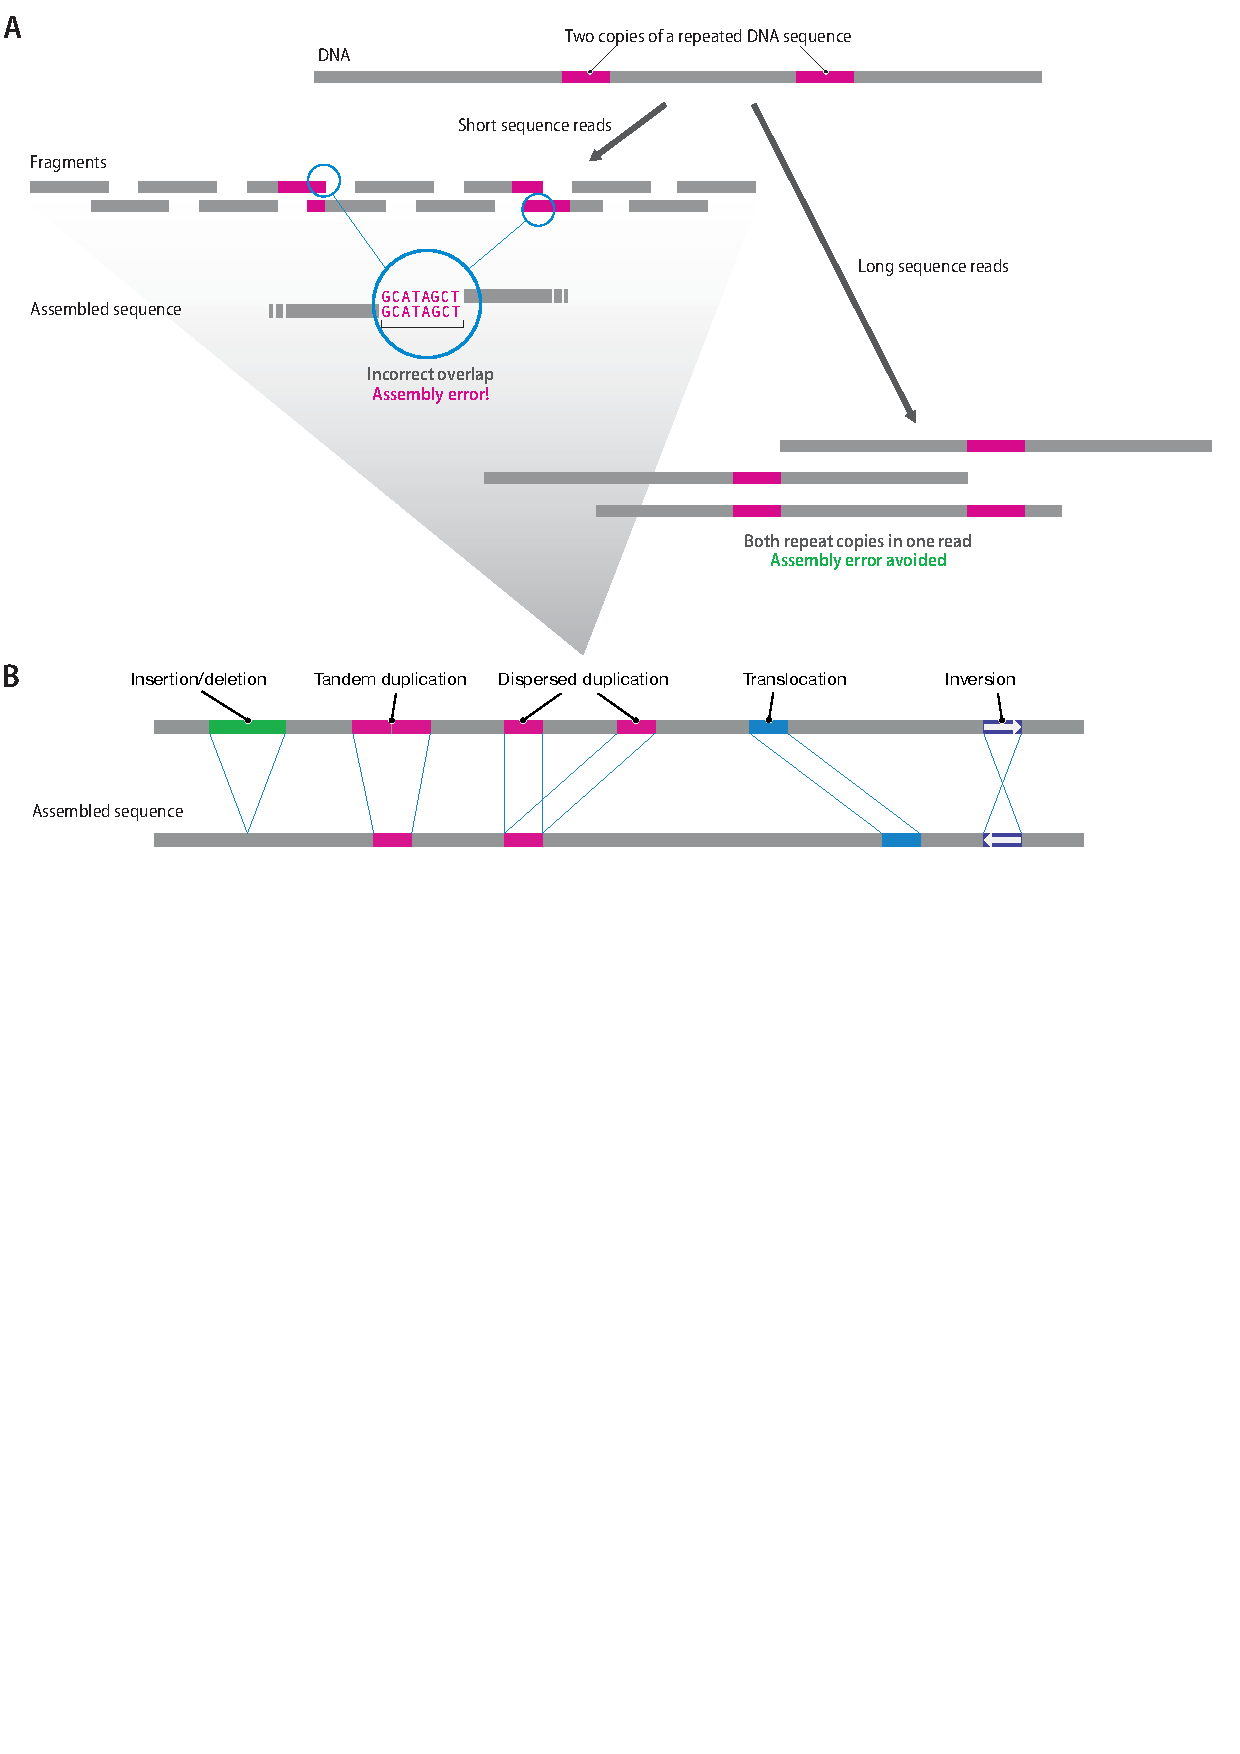
\includegraphics[width=\textwidth]{img/fig_1.pdf}
    \vspace{0.25cm}
    \caption[Limitaciones del ensamblaje genómico con lecturas cortas]{Limitaciones 
    del ensamblaje genómico con lecturas cortas. (\textbf{A}) Si una secuencia 
    contiene una duplicación dispersa de, por ejemplo, $\sim$500 pb y secuenciamos
    con lecturas cortas ($\sim$100 pb), herramientas de alineamiento pueden superponerlas 
    como una sola copia. Con lecturas largas ($\sim$10 kb), ambas copias se capturan 
    en una única lectura, resolviendo correctamente la duplicación. (\textbf{B}) 
    Esta dificultad se extiende a todos los tipos de SVs; inserciones, deleciones,
    duplicaciones, traslocaciones, inversiones o combinaciones de ellas. Adaptado
    de \cite{brown_genomes_2023}.}
    \label{fig:fig_1}
\end{figure}

Las tecnologías de secuenciación de lectura larga surgieron hace una década, 
marcando un punto de inflexión en el ensamblaje de secuencias al abordar las 
limitaciones de las lecturas cortas. Inicialmente, estas tecnologías tenían tasas 
de error mucho más elevadas ($\sim$10\%) en comparación con las lecturas cortas 
(< 1\%) \cite{espinosa_advancements_2024}. Si bien esto permitió el ensamblaje rutinario de genomas 
bacterianos, limitó su aplicación en genómica humana, particularmente para la 
detección de mutaciones puntuales \cite{loman_complete_2015}. Sin embargo, las 
mejoras continuas en las plataformas de secuenciación de lectura larga han reducido 
progresivamente estas tasas de error, permitiendo finalmente la generación del primer genoma de 
referencia humano sin huecos, conocido como ensamblaje telómero a telómero (T2T) 
\cite{nurk_complete_2022}. Este logro resolvió regiones genómicas previamente 
inaccesibles que permanecían incompletas en la versión 38 del genoma de referencia 
humano del Consorcio de Referencia Genómica (GRCh38) (ver \textbf{Figura \ref{fig:T2T_ref}}).

Más allá de las diferencias metodológicas de secuenciación, existen disparidades 
significativas entre las plataformas de lectura larga en términos de 
accesibilidad y coste. Aunque PacBio fue pionera en este campo en 2011 con 
sistemas de secuenciación de alto rendimiento, sus plataformas han requerido 
consistentemente inversiones de cientos de miles de dólares. En contraste, el 
lanzamiento del MinION por parte de ONT en 2014 supuso un cambio de paradigma al 
introducir un dispositivo portátil de bajo rendimiento con una inversión de 
apenas unos pocos miles de dólares \cite{espinosa_advancements_2024,noauthor_vega_nodate}. 

Posteriormente, ONT amplió su catálogo hacia la gama de alto rendimiento con los 
dispositivos PromethION, cuyo modelo de entrada ``P2 solo'' permite la secuenciación 
de genomas completos (WGS) mediante conexión a ordenador por menos de 20.000 
dólares. Esto ha hecho que la secuenciación de lectura larga sea económicamente 
accesible para la mayoría de laboratorios de biología molecular, desplazando el 
principal obstáculo hacia la formación especializada en bioinformática necesaria 
para el procesamiento y análisis de los datos generados \cite{oxford_nanopore_technologies_nanopore_nodate}.

La tecnología de secuenciación de ONT funciona mediante la medición de cambios 
en la corriente iónica a medida que moléculas individuales de ADN o ARN son 
translocadas por una enzima de desenrollamiento anclada a la superficie del 
nanoporo. Estos nanoporos están dispuestos en arrays sobre una celda de flujo
(\textit{flowcell}), el componente consumible fundamental de ONT, que alberga 
miles de canales de detección independientes. Los cambios individuales de corriente 
en cada nanoporo se interpretan mediante un modelo basado en redes neuronales 
entrenado con secuencias nucleotídicas sintéticas de contenido conocido y sus 
correspondientes variaciones de corriente, permitiendo determinar la secuencia 
de cada molécula que atraviesa el nanoporo (\textit{basecalling}) \cite{mardis_tracing_2025}.

Las mejoras recientes en la arquitectura de los nanoporos de las celdas de flujo 
(con la transición de la proteína de poro R9, con constricción de 9 Å, a la 
variante R10 que incorpora un barril elongado y constricción de 10 Å) y de los 
algoritmos de basecalling han mejorado significativamente la precisión de esta
técnica de secuenciación (\textbf{Figura~\ref{fig:ont_pores}}). Esto hace de la 
secuenciación por nanoporos un enfoque viable para el análisis sistemático de 
variantes asociadas a cáncer; incluyendo la reconstrucción de SVs, modificaciones
epigenéticas como metilaciones sin tratamientos adicionales como la conversión
por bisulfito, así como la asignación directa de estas variantes a sus respectivos 
cromosomas parentales (\textit{haplotype phasing}) 
\cite{kolmogorov_scalable_2023,sakamoto_phasing_2022,schaal_migrating_2022}.

\section{Variación estructural en cáncer}

Según el Instituto Nacional del Cáncer (NCI), el cáncer comprende más de 100 tipos 
diferentes que se originan cuando células normales experimentan alteraciones 
genéticas y/o epigenéticas que resultan en proliferación descontrolada y 
la alteración de la homeostasis del organismo \cite{noauthor_what_2007,hanahan_hallmarks_2011}. 
El desarrollo tumoral representa un proceso complejo producto de las interacciones entre el 
genotipo individual y diversos factores ambientales, impulsando una evolución 
clonal en la que diferentes subpoblaciones de células malignas compiten por 
recursos y espacio \cite{turajlic_resolving_2019}. La secuenciación del ADN 
tumoral permite la identificación de mutaciones \textit{driver} específicas de 
cada paciente, facilitando la selección e implementación más efectiva de terapias 
dirigidas \cite{sicklick_molecular_2019}.

La importancia de las variantes estructurales (SVs) como \textit{hallmark} del 
cáncer es cada vez más evidente. Un análisis reciente de 2.658 genomas tumorales 
reveló que aproximadamente el 50\% de las mutaciones \textit{driver} se solapan con 
SVs, destacando su papel crucial en el desarrollo del cáncer 
\cite{li_patterns_2020,menghi_tandem_2018}. A pesar de su importancia como 
biomarcadores en enfermedades oncológicas, nuestro conocimiento sobre las SVs sigue siendo limitado en comparación con las variantes 
de nucleótido único (SNVs). Esta brecha de conocimiento se debe principalmente a 
las limitaciones técnicas de la secuenciación de lectura corta, que ha dominado 
los proyectos de secuenciación genómica a gran escala. Utilizando lecturas cortas, 
la detección de SVs se basa principalmente en estimaciones de variaciones en el 
número de copias (CNVs), una medida indirecta que no logra capturar eventos 
como inversiones o translocaciones balanceadas 
\cite{cameron_comprehensive_2019,abel_mapping_2020}.

El equipo de investigación en secuenciación por nanoporos de la Unidad de 
Bioinformática del Centro Nacional de Investigaciones Oncológicas desarrolla, 
entre sus líneas prioritarias, análisis de genomas completos de pacientes con 
mieloma múltiple (MM) en estadios pre y post-tratamiento \cite{haertle_multi-omic_2026}. 
El MM es una neoplasia de células B terminalmente diferenciadas (células plasmáticas) 
caracterizada por translocaciones cromosómicas frecuentes que sitúan oncogenes 
bajo el control de potenciadores de expresión de inmunoglobulinas, así como por 
la adquisición de otras SVs de gran tamaño. Algunas de estas alteraciones, 
descritas por primera vez hace más de dos décadas, siguen siendo los 
principales marcadores pronósticos y son detectadas principalmente mediante 
hibridación fluorescente in situ (FISH) \cite{kuehl_multiple_2002}.

El MM sigue un patrón característico de remisión-recaída donde las células 
malignas adquieren progresivamente resistencia a múltiples líneas terapéuticas 
(\textbf{Figura~\ref{fig:evo_MM}}) \cite{kurtin_relapsed_2013}. En este contexto, la secuenciación por 
nanoporos de ONT junto con métodos automatizados de llamada de SVs podría ampliar 
nuestra comprensión de los mecanismos fisiopatológicos e identificar potencialmente 
nuevos marcadores pronósticos y objetivos terapéuticos, contribuyendo en última 
instancia a mejorar el manejo clínico y el pronóstico de supervivencia. 

\begin{figure}[H]
    \centering
    \includegraphics[width=0.7\textwidth]{img/evo_MM.png}
\caption[Ciclo de remisión-recaída del mieloma múltiple]{Ciclo de 
    remisión-recaída del mieloma múltiple. Se caracteriza por 
    ciclos sucesivos de respuesta, remisión y recaída bajo tratamiento, 
    monitorizados mediante niveles de proteína M (anticuerpo anómalo 
    producido por células plasmáticas malignas). Las recaídas sucesivas 
    acumulan SVs que generan evolución clonal con respuestas progresivamente 
    más breves y superficiales. Cortesía de Álvaro Otero Sobrino, Hospital 12 de Octubre.}
    \label{fig:evo_MM}
\end{figure}

\section{Justificación del proyecto}

En la última guía de recomendaciones para la bioinformática en la práctica 
clínica publicada en \textit{Genome Medicine}, los autores reconocen el valor de 
la secuenciación de lecturas largas para la detección de SVs, aunque también 
señalan la necesidad de establecer estándares consensuados por la comunidad 
científica respecto a las herramientas de detección de CNVs y SVs. Sin embargo, 
la evaluación de estos métodos sigue siendo compleja debido principalmente a la 
ausencia de \textit{datasets} curados y abiertos \cite{lavrichenko_recommendations_2025}.

La generación de modelos celulares que incorporen de manera estable conjuntos 
de SVs requeriría la implementación de procedimientos experimentales complejos, 
con una considerable inversión de tiempo y recursos económicos. Por el contrario, 
la utilización de datos sintéticos constituye una alternativa económicamente 
viable que, además, presenta la ventaja de conocer a priori la verdad absoluta, 
facilitando así la validación y evaluación de los métodos desarrollados.

Los datos experimentales son esenciales para crear y mejorar métodos 
computacionales, cuyos resultados no solo proporcionan nuevos conocimientos, 
sino que también pueden servir como base para refinar futuros experimentos. No
obstante, los datos sintéticos pueden ayudar a catalizar este ciclo, generando información más 
rápidamente y con un menor consumo de recursos.

    \chapter{Objetivos}

Este proyecto se centró en la evaluación de enfoques mediante secuenciación 
de lectura larga por nanoporos para rastrear y analizar variaciones 
estructurales somáticas a lo largo de la evolución de genomas oncológicos. Con 
este fin, se establecieron los siguientes objetivos específicos:

\begin{enumerate}
    \item Evaluar la capacidad de los datos de secuenciación WGS de lecturas 
    largas obtenibles con una única celda de flujo de ONT PromethION, en 
    combinación con diferentes longitudes medias de lecturas, para la 
    reconstrucción de variantes estructurales de gran tamaño que abarcan 
    bandas cromosómicas completas mediante alineamiento a un genoma T2T.

    \item Comparar detectores de variantes estructurales actuales considerando 
    precisión de detección y eficiencia computacional, con especial atención 
    a capacidades de clasificación y demandas de recursos, para identificar 
    soluciones óptimas en flujos de trabajo de análisis rutinarios.

    \item Explorar el potencial de la secuenciación de lectura larga por 
    nanoporos para detectar marcadores genómicos relevantes en Mieloma 
    Múltiple más allá de los tradicionalmente identificados por FISH, y 
    evaluar estrategias complementarias para mejorar la caracterización de 
    alteraciones cromosómicas.
\end{enumerate}
    \blankpage{}

    \chapter{Material y métodos}

\section{Recursos computacionales}

El desarrollo del código para este proyecto se llevó a cabo en un MacBook Pro 
con un procesador M4 Pro, que incluye una CPU de 14 núcleos, una GPU de 20 
núcleos, 24 GB de memoria unificada y 1 TB de almacenamiento SSD.

Debido a las demandas computacionales de las tareas requeridas para lograr los 
objetivos propuestos, se utilizó el clúster de computación de alto rendimiento 
(HPC) del CNIO. Esta infraestructura cuenta actualmente con 12 nodos de cómputo 
cuyas configuraciones se detallan en la \textbf{Tabla~\ref{tab:nodes}}.

\vspace{0.50cm}

\begingroup
\footnotesize
\setlength{\LTpre}{0pt}
\setlength{\LTpost}{0pt}
\begin{longtable}{>{\RaggedRight\arraybackslash}p{1.75cm} 
                  >{\RaggedRight\arraybackslash}p{2.75cm} 
                  >{\RaggedRight\arraybackslash}p{2.25cm}
                  >{\RaggedRight\arraybackslash}p{2cm}
                  >{\RaggedRight\arraybackslash}p{4cm}}
    \caption[Especificaciones técnicas de los nodos del clúster HPC del CNIO]{Especificaciones técnicas 
    del los nodos del clúster HPC del CNIO \cite{tomas_di_domenico_cluster_nodate}.}\vspace{0.30cm}\label{tab:nodes}\\
    \toprule
    \textbf{Cantidad} & \textbf{Identificadores} & \textbf{núcleos CPU} & \textbf{RAM} & \textbf{GPUs} \\ 
    \midrule
    \endfirsthead
    
    \multicolumn{5}{@{}l}{\RaggedRight \textbf{\tablename\ \thetable{}} -- Continued} \\
    \\
    \toprule
    \textbf{Cantidad} & \textbf{Identificadores} & \textbf{núcleos CPU} & \textbf{RAM} & \textbf{GPUs} \\ 
    \midrule
    \endhead
    \\
    \midrule 
    \multicolumn{5}{r}{Continued on next page} \\
    \endfoot
    
    \bottomrule
    \endlastfoot
    
    \\
    1     & bc001      & 24  & 32 GB  & -- \\
    \\
    6     & bc00[2-7]  & 52  & 512 GB & -- \\
    \\
    3     & bc00[8-10] & 128 & 1 TB   & -- \\
    \\
    1     & hm001      & 224 & 2 TB   & -- \\
    \\
    1     & gp001      & 112 & 768 GB & 3 x Nvidia A100 80 GB \\
    \\
    
\end{longtable}
\endgroup

Los recursos de almacenamiento del clúster incluyen 52 TB de espacio estándar 
para los directorios de inicio de los usuarios, además de 512 TB de 
almacenamiento de alto rendimiento optimizado para las operaciones de entrada y 
salida de los trabajos de cálculo. De este almacenamiento de alto rendimiento, 
se asignaron específicamente 15 TB para la ejecución de código y la generación 
de datos asociados a este proyecto.

\section{Herramientas de software}

Positron fue utilizado como interfaz principal para el acceso al clúster a través 
de protocolo SSH (\textit{Secure Shell}) y el desarrollo de código. Se utilizaron 
principalmente los lenguajes de programación Bash, Python y R.

El clúster opera bajo el gestor de tareas Slurm, un sistema basado en Linux/Unix 
para la gestión de recursos de HPC. La integración de los flujos de trabajo se 
logró mediante Snakemake, un administrador que permite ejecutar análisis 
reproducibles y escalables a través de la definición de reglas basadas en Python. 
La instalación del software para cada regla se realizó mediante ambientes Conda, 
lo que evita instalar software en cada nodo del clúster donde se ejecuten los 
trabajos y posibles problemas de compatibilidad entre los diferentes programas. 
Para gestionar los ambientes Conda, se utilizó Miniforge, una distribución 
ligera a la que se incluyó el repositorio Bioconda para descargar herramientas 
especializadas en bioinformática.

En la \textbf{Tabla~\ref{tab:software}} se recogen todas las herramientas de 
software utilizadas en este trabajo. En las siguientes secciones de este apartado 
se describe cómo se han integrado las distintas herramientas para crear los 
flujos de trabajo necesarios para alcanzar los objetivos específicos de este 
proyecto. 

\subsection{Simulación de datos de secuenciación de lecturas largas con eventos
estructurales y detección de variantes}

\subsubsection{Simulador de datos}

Para la simulación específica de haplotipos con variantes estructurales simples 
y complejas, se seleccionó el set de herramientas VISOR. Su módulo VISOR 
LASeR incluye un modelo de incorporación de errores entrenado con lecturas de ONT 
R10.4.1, proporcionado por Badread \cite{wick_badread_2019}.

\subsubsection{Detectores de variantes estructurales}

Se seleccionó un conjunto de herramientas de detección de SV en base a dos 
criterios clave: compatibilidad con lecturas largas de ONT y capacidad de 
detección de SV somáticas. Cada herramienta seleccionada presenta 
características distintivas e interesantes para los análisis:

\begin{itemize}

    \item \textbf{SAVANA}: implementa un modelo de aprendizaje automático 
    entrenado con muestras pareadas tumor-normal para detectar SV somáticas y 
    aberraciones en el número de copias (CNAs) en casos clínicos.

    \item \textbf{Severus}: especializado en análisis comparativos tumor/normal, 
    admite múltiples muestras tumorales y emplea marcos de grafos de puntos de 
    ruptura para la detección de reordenamientos cromosómicos complejos.

    \item \textbf{Sniffles2}: una herramienta pionera de detección de SV en 
    lecturas largas de ONT desde 2018, manteniéndose en desarrollo continuo y con 
    actualizaciones regulares.

    \item \textbf{SVision-pro}: emplea un enfoque basado en redes neuronales que 
    convierte características genómicas de muestras pareadas en representaciones 
    de imágenes para la detección comparativa de SV.

\end{itemize}

\subsubsection{Flujo de trabajo para la generación y detección de variantes 
estructurales}

Se desarrolló un flujo de trabajo integral para simulaciones basadas en VISOR y 
el posterior análisis de detección de variantes estructurales. Las etapas principales
del proceso se muestran en la \textbf{Figura \ref{fig:visor-sim}}. El código fuente 
y la documentación asociada están disponibles en el siguiente repositorio: 
\url{https://github.com/villena-francis/visor-simulations}.

\begin{figure}[!htbp]
    \centering
    \includegraphics[scale=1.25]{img/visor-simulations.pdf}
    \captionsetup{labelfont=bf, textfont={normalsize,it}}
    \caption[Versión simplificada del flujo de trabajo ``visor-simulations'' para 
    la simulación de lecturas largas y la detección de SVs]{Versión simplificada 
    del flujo de trabajo ``visor-simulations'' para la simulación de lecturas 
    largas y la detección de SVs. VISOR-HACk genera archivos FASTA (secuencias
    molde) con SVs incorporadas utilizando un genoma de referencia e
    instrucciones de haplotipos en formato BED (coordenadas genómicas delimitadas 
    por tabulaciones). El script makeBED crea un archivo BED (intervalos genómicos) 
    a partir de los tamaños máximos de cromosomas extraídos de los FASTA de haplotipos. 
    Posteriormente, VISOR-LASeR genera archivos BAM (lecturas de secuenciación 
    alineadas) junto con sus índices (.bai), empleando como entrada los ficheros
    obtenidos en los pasos anteriores. Finalmente, las lecturas alineadas son 
    procesadas por los detectores de SVs, generando cada uno su correspondiente 
    archivo VCF (Variant Call Format) con las SVs identificadas.}
    \label{fig:visor-sim}
\end{figure}

\subsubsection{Configuración de las simulaciones}

En cada simulación de secuenciación de genoma completo mediante ONT, se 
introdujeron SVs en el genoma de referencia T2T-CHM13 (\textit{chm13v2.0\_maskedY\_rCRS.fa}), 
para generar lecturas sintéticas con una cobertura media de 40x. Con el objetivo de 
evaluar el efecto de la longitud de las lecturas sobre la eficiencia del mapeo al genoma de 
referencia y la capacidad de detección de las SVs introducidas, se realizaron 
simulaciones con cuatro longitudes medias de lecturas: 15, 30, 50 y 100 kb. Para 
cada longitud, se generó una muestra normal (sin SVs) y tres réplicas tumorales, 
generándose así 12 muestras en total.

El conjunto de SVs utilizadas se basó en aberraciones cromosómicas características 
de mieloma múltiple, algunas descritas en la literatura científica y otras 
observadas en pacientes reales (\textbf{Tabla~\ref{tab:stagesV1}}). Dado que los 
puntos de rotura específicos no se encuentran detallados en la literatura 
clínica para el genoma de referencia T2T-CHM13, sus coordenadas se determinaron 
de forma aproximada utilizando el navegador genómico UCSC Genome Browser.

\begingroup
\vspace{0.50cm}

\footnotesize

\begin{longtable}{>{\RaggedRight\arraybackslash}p{2.25cm} 
                  >{\RaggedRight\arraybackslash}p{10cm} 
                  >{\RaggedLeft\arraybackslash}p{2cm}}
    \captionsetup{labelfont=bf, textfont={normalsize,it}}
    \caption[Características de las SVs simuladas]{Características de las SVs 
    simuladas, inspiradas en datos de MM. \cite{aksenova_genome_2021}. Los valores 
    de tamaño representan la longitud final en pares de bases (pb) tras la inserción en 
    el genoma, aquellos marcacados con * implican puntos de rotura en regiones centroméricas. La 
    duplicación en tándem consiste en un fragmento de 2 030 586 pb 
    repetido cuatro veces. Los archivos de entrada para la simulación de estas
    lecturas con \textit{visor-simularions} están disponibles en 
    \url{https://github.com/villena-francis/tfe_unir/tree/main/data/cluster_bmk/visor_v1}.}
    \vspace{0.3cm}\label{tab:stagesV1}\\

    \toprule
    \textbf{Tipo de SV} & \textbf{Descripción} & \textbf{Tamaño (pb)} \\ 
    \midrule
    \endfirsthead
    
    \multicolumn{3}{@{}l}{\RaggedRight \textbf{\tablename\ \thetable{}} -- Continued} \\
    \\
    \toprule
    \textbf{SV type} & \textbf{Description} & \textbf{Size (pb)} \\ 
    \midrule
    \\
    \endhead
    \\
    \midrule 
    \multicolumn{3}{r}{\footnotesize Continued on next page} \\
    \endfoot
    
    \bottomrule
    \endlastfoot

    \\
    Duplicación en tandem             & Ganancia de un brazo 1q extra, una de las anomalías citogenéticas estructurales más frecuentes en el MM. & 123600854* \\
    \\
    Duplicación en tandem             & Amplificación de 1q21, otra de las anomalías estructurales asociadas a progresión de MM.                 & 11997705 \\
    \\
    Deleción                          & Deleción del 17p (~10\% de casos), indicador de mal pronóstico. La región mínima delecionada en 17p13 incluye el gen supresor tumoral \textit{TP53}. & 4307895 \\
    \\
    Deleción                          & Deleción total del 17p, también observado en células con MM.   & 23892418* \\
    \\
    Deleción                          & Perdida de una copia completa del cromosoma 13, también frecuente en MM  &  113566675 \\
    \\
    Translocación recíproca           & Reordenamiento cromosómico que afecta al gen de la cadena pesada de inmunoglobulina (\textit{IGH}) en 14q32, la más frecuente es con 11q13.                                                 & 500000  \\
    \\
    Translocación (cortar-pegar)      & Reordenamiento que afecta a \textit{CDKN2A}, gen supresor tumoral crucial cuya inactivación mediante mutaciones o deleciones es una de las alteraciones más frecuentes en cánceres humanos, solo superada por alteraciones en \textit{TP53}. & 50000 \\
    \\
    Inversión                         & Inversión cromosómica en 6q25.1, incluida como variante control para validar las capacidades de los detectores de SVs, aunque no es típicamente característica en mieloma múltiple.          & 3600000  \\
    \\

\end{longtable}
\endgroup

\subsection{Análisis comparativo de detectores de variantes estructurales}

\subsubsection{Marco de evaluación}

La evaluación del rendimiento se basó en un marco de clasificación binaria 
que categorizó los resultados de detección de SVs como:

\begin{itemize}
    \item \textbf{Verdaderos Positivos (VP)}: SVs simuladas que fueron detectadas 
    correctamente.

    \item \textbf{Falsos Positivos (FP)}: SVs identificadas por el detector pero 
    ausentes en la simulación, verificadas mediante inspección de lecturas.

    \item \textbf{Falsos Negativos (FN)}: SVs simuladas presentes en las lecturas 
    pero no detectadas por el detector.
\end{itemize}

Los Verdaderos Negativos (VN) fueron excluidos de este análisis debido a su falta 
de aplicabilidad en la evaluación de la detección de SVs, dado el extenso 
espacio genómico y la naturaleza de los métodos de detección de variantes 
estructurales.

\subsubsection{Métricas de rendimiento}

Dada la imposibilidad de cuantificar los VN, se seleccionaron métricas 
independientes de esta categoría para evaluar el rendimiento de los detectores
de SVs:

\begin{itemize}
    \item \textbf{Sensibilidad} (\textit{Recall}): Proporción de casos positivos correctamente 
    identificados
    \begin{equation}
        \label{eq:recall}
        Recall = \frac{VP}{VP + FN}
    \end{equation}

    \item \textbf{Precisión} (\textit{Precision}): Exactitud de las predicciones positivas
    \begin{equation}
        \label{eq:precision}
        Precision = \frac{VP}{VP + FP}
    \end{equation}

    \item \textbf{Puntuación F1} (\textit{F1 Score}): Media armónica de la precisión (P) y la sensibilidad (S)
    \begin{equation}
        \label{eq:f1score}
        F1 = 2 \cdot \frac{P \cdot S}{P + S}
    \end{equation}
\end{itemize}

Adicionalmente, se evaluó la eficiencia computacional de cada detector mediante 
las estadísticas generadas por el gestor de recursos Slurm, incluyendo: 

\begin{itemize}
    \item \textbf{Utilización de CPU/GPU} (número de núcleos)
    
    \item \textbf{Consumo de memoria RAM} (GB)
    
    \item \textbf{Tiempo de ejecución} (minutos)
\end{itemize}

\subsubsection{Herramientas de validación y análisis}

La visualización de las lecturas alineadas se realizó utilizando Genome-Wide (GW), 
un navegador genómico avanzado que permite navegar de forma instantánea y fluida 
a pesar del elevado volumen de los ficheros BAM (más de 100 GB cada uno). Este navegador 
facilita la curación manual mediante navegación ágil entre variantes anotadas en 
los VCF generados por los detectores de SVs, permitiendo validar los hallazgos 
(\textbf{Figura~\ref{fig:GW_UI}}).

Dado que el clúster carece de soporte para la ejecución de herramientas con 
interfaz gráfica, el directorio que contenía los ficheros BAM generados por las 
simulaciones se montó en un equipo local utilizando el protocolo SSHFS 
(\textit{Secure SHell FileSystem}).

Para el cálculo automatizado de las métricas descritas, se revisaron manualmente
todas las lecturas, considerando únicamente las SVs que pudieron ser reconstruidas exitosamente 
tras el alineamiento de las lecturas al genoma de referencia.    

\subsubsection{Procesamiento y visualización de resultados}

El procesamiento de los resultados, el cálculo comparativo de métricas y la 
generación de representaciones gráficas se llevaron a cabo mediante scripts 
desarrollados en R. El código completo está disponible en el repositorio 
asociado a este proyecto: 
\url{https://github.com/villena-francis/tfe_unir/tree/main/data/cluster_bmk/stats_plots.R}.
    \blankpage{}

    \chapter{Resultados}

\section{Demandas computacionales de las simulaciones de lecturas largas}

Las simulaciones realizadas con VISOR generaron un total de 4.54 TB de datos 
sintéticos de secuenciación de lecturas largas mediante ONT. De este 
volumen total, aproximadamente 2.54 TB correspondieron a lecturas alineadas al 
genoma de referencia en formato BAM y sus respectivos ficheros índice, mientras 
que el volumen restante consistió en lecturas no alineadas en formato FASTQ 
(\textbf{Tabla~\ref{tab:file_sizes}}). Los datos de uso de CPUs, consumo de 
memoria RAM y los tiempos de ejecución se muestran en la 
\textbf{Figura~\ref{fig:hpc_visor_laser}}.

\begin{figure}[H]
    \centering
    \includegraphics[width=\textwidth]{data/cluster_bmk/hpc_visor_laser.pdf}
    \caption[Demanda de recursos computacionales del módulo VISOR LASeR]{Demanda 
    de recursos computacionales del módulo VISOR LASeR en función de la 
    longitud de lecturas. Los gráficos muestran el consumo de núcleos de CPU 
    (\textbf{a}), el uso de memoria RAM (\textbf{b}) y el tiempo de ejecución 
    (\textbf{c}) para longitudes de lectura de 15, 30, 50 y 100 Kb. Se 
    generaron tres réplicas técnicas WGS de tipo ``tumoral'' y una de tipo 
    ``normal'' para cada longitud, todas con una profundidad de secuenciación 
    de 40x. No se incluyen cálculos para el módulo VISOR HACk, ya que se 
    ejecuta una única vez durante pocos minutos con bajo consumo de recursos 
    para incorporar el conjunto de variantes estructurales en el genoma de 
    referencia que posteriormente alimentará a VISOR LASeR. Los datos en bruto 
    están disponibles en \url{https://github.com/villena-francis/tfe_unir/tree/main/data/cluster_bmk/hpc_data}.}
    \label{fig:hpc_visor_laser}
\end{figure}

\section{Detección de variantes estructurales}

\subsection{Exploración de los alineamientos de lecturas largas generados}

De las SVs incluidas en las instrucciones para la generación de los datos 
sintéticos (\textbf{Tabla~\ref{tab:stagesV1}}), se identificaron mediante 
inspección visual con GW los breakpoints asociados a la duplicación en tándem 
de 1q21 (\textbf{Figura~\ref{fig:chr1_del1q21}}), la inversión cromosómica de 6q25.1 
(\textbf{Figura~\ref{fig:chr6_inv6q25.1}}), la translocación de 
cortar-pegar de un fragmento de la región 9p21.3 (\textbf{Figura~\ref{fig:chr9_del9p21.3}}), 
la translocación recíproca entre 11q13 y 14q32 (\textbf{Figura~\ref{fig:chr11-14_translocation}}), 
y la deleción de 17p13 (\textbf{Figura~\ref{fig:chr17_del17p13}}). En relación a las 
SVs de mayor tamaño (la ganancia de 1q, la deleción de 17p y la pérdida de una 
copia del chr13), solo pudieron inferirse la pérdida del chr13 completo y la 
deleción del 17p mediante la representación gráfica de los valores 
de cobertura (\textbf{Figura~\ref{fig:chromosomes_comparison}}).

\begin{figure}[H]
    \centering
    \begin{subfigure}[b]{\textwidth}
        \centering
        \caption{chr1}
        \includegraphics[width=0.64\textwidth]{data/cluster_bmk/calls_data/chr1_40x_15000_A.png}
        \label{fig:chr1_subfig}
    \end{subfigure}
    
    \begin{subfigure}[b]{\textwidth}
        \centering
        \caption{chr13}
        \includegraphics[width=0.64\textwidth]{data/cluster_bmk/calls_data/chr13_40x_15000_A.png}
        \label{fig:chr13_subfig}
    \end{subfigure}
    
    \begin{subfigure}[b]{\textwidth}
        \centering
        \caption{chr17}
        \includegraphics[width=0.64\textwidth]{data/cluster_bmk/calls_data/chr17_40x_15000_A.png}
        \label{fig:chr17_subfig}
    \end{subfigure}
    
    \caption[Perfiles de profundidad de cobertura cromosómica]{Perfiles de 
    profundidad de cobertura cromosómica. (\textbf{a}) chr1: se observa la 
    amplificación de la región 1q21, mientras que el resto del cromosoma mantiene 
    cobertura normal excepto en la región centromérica; (\textbf{b}) chr13: la cobertura 
    reducida a aproximadamente la mitad (20x) refleja la pérdida de una copia 
    del cromosoma completo. La región 13p12 muestra cobertura nula debido a 
    duplicaciones segmentales (LCR13) que impiden el alineamiento único de las 
    lecturas; (\textbf{c}) chr17: la cobertura reducida a la mitad en 17p evidencia la 
    deleción de este brazo cromosómico. La región 17p12 muestra cobertura nula 
    debido a duplicaciones segmentales (CMT1A-REPs) que impiden el alineamiento 
    único de las lecturas. Los datos corresponden a la muestra tumoral A con 
    longitud media de lectura de 15 kb. Los gráficos fueron generados 
    utilizando la herramienta Wakhan.}
    \label{fig:chromosomes_comparison}
\end{figure}

\subsection{Formato de los arcivos de salida}

Los detectores de SVs generan archivos VCF similares a los producidos por los 
detectores de SNVs. Sin embargo, en estos casos cada fila representa uno de los 
puntos de ruptura (\textit{breakpoint}) que delimitan las SVs en cuestion. Las 
variantes estructurales simples, como inserciones o deleciones, requieren la 
identificación de dos puntos de ruptura, mientras que las variantes complejas, 
como las translocaciones recíprocas, necesitan la detección de cuatro puntos de 
ruptura. A modo ilustrativo, los archivos de salida finales generados por cada 
detector, correspondientes a una de las muestras simuladas están disponibles en 
\url{https://github.com/villena-francis/tfe_unir/tree/main/data/cluster_bmk/calls_data/raw}.

En el caso de \textbf{SAVANA}, se observa una limitación significativa en su 
archivo VCF de salida en comparación con otros detectores de variantes: su 
incapacidad para clasificar los tipos de variantes estructurales. Esta 
herramienta únicamente identifica y correlaciona puntos de ruptura sin 
proporcionar información sobre el tipo específico de variante estructural 
presente en cada caso.

Por su parte, \textbf{Severus} va más allá de la detección convencional de 
variantes estructurales al incorporar un procesamiento especializado para 
repeticiones en tándem de número variable (VNTRs, del inglés \textit{Variable 
Number Tandem Repeats}), lo que permite una anotación precisa de las variantes 
estructurales dentro de estas regiones. La herramienta proporciona una salida 
integral que incluye archivos VCF estándar, métricas detalladas de calidad en 
archivos de registro (\textit{log}), y representaciones gráficas de los 
reordenamientos cromosómicos mediante gráficos de visualización.

En cuanto a \textbf{Sniffles2}, este detector genera exclusivamente archivos 
VCF estándar, sin archivos de soporte adicionales ni visualizaciones 
complementarias. No obstante, al igual que Severus, también incorpora 
funcionalidades para mejorar la detección en regiones con VNTRs para optimizar 
la precisión en la detección de variantes asociadas a estas regiones del genoma.

Finalmente, \textbf{SVision-pro}, a pesar de utilizar un enfoque innovador 
basado en codificación de imágenes para analizar características genómicas y 
detectar variaciones inter-genómicas entre muestras pareadas tumor-normal, 
limita su salida a archivos VCF estándar en los que las variantes no aparecen 
ordenadas secuencialmente por cromosoma ni por sus coordenadas genómicas. Las 
representaciones visuales empleadas en su pipeline de procesamiento interno no 
son accesibles al usuario como ficheros de salida.  

\subsection{Rendimiento}

El análisis comparativo del rendimiento de los cuatro métodos de detección de 
variantes estructurales reveló diferencias significativas en términos de precisión, 
sensibilidad y tasa de falsos positivos. 

\begin{figure}[H]
    \centering
    \includegraphics[width=\textwidth]{data/cluster_bmk/perform_calls.pdf}
    \caption[Rendimiento de los métodos de detección de variantes estructurales 
    evaluados]{Rendimiento de los métodos de detección de variantes estructurales 
    SAVANA, Severus, Sniffles2 y SVision-pro, basado en las métricas de precisión, 
    exhaustividad (\textit{recall}) y puntuación F1. Para cada profundidad de 
    secuenciación, se obtuvieron tres resultados por métrica mediante la comparación 
    de una muestra normal contra tres réplicas técnicas de la muestra tumoral. Los 
    datos en bruto utilizados para todos los cálculos están disponibles en 
    \url{https://github.com/villena-francis/master_thesis/tree/main/data/cluster_bmk/calls_data/callings.csv}.}
    \label{fig:perform_calls}
\end{figure}

\textbf{SAVANA} demostró el mejor desempeño global con un F1-score promedio de 0.977 ± 0.041, 
manteniendo una precisión del 95.8\% y una sensibilidad del 100\%, detectando 
consistentemente las cinco SVs esperadas (duplicación de 1q21, inversión de 6q25.1, 
translocación de 9p21.3, translocación recíproca 11q13-14q32 y deleción de 17p13) 
en todas las réplicas y longitudes de lectura evaluadas, con un promedio de solo 
0.25 falsos positivos por análisis. 

\textbf{Severus}, aunque alcanzó una sensibilidad perfecta (100\%) detectando todas las 
SVs esperadas, presentó una precisión notablemente inferior (21.8\% ± 5.8\%) 
debido a una alta tasa de falsos positivos (promedio de 19.25 por análisis), 
resultando en un F1-score de 0.355 ± 0.076. 

\textbf{SVision-pro} detectó correctamente cuatro de las cinco SVs (inversión de 6q25.1, 
translocaciones de 9p21.3 y 11q13-14q32, y deleción de 17p13), alcanzando una 
sensibilidad del 80\%, pero su rendimiento estuvo severamente comprometido por 
un número excepcionalmente elevado de falsos positivos (promedio de 546.2), lo 
que redujo drásticamente su precisión a 0.7\% ± 0.1\% y su F1-score a 0.014 ± 0.001. 

\textbf{Sniffles2} mostró el peor desempeño general, detectando únicamente la translocación 
recíproca 11q13-14q32 en el 50\% de las réplicas, con una sensibilidad promedio 
del 10\% ± 10.4\%, precisión del 2.1\% ± 2.4\%, y F1-score de 0.035 ± 0.038. 

Estos resultados indican que SAVANA ofrece el mejor balance entre sensibilidad 
y precisión para la detección de SVs en datos de secuenciación de lectura larga, 
mientras que los otros métodos requieren optimización adicional de parámetros o 
filtrado post-procesamiento para reducir los falsos positivos y mejorar su 
aplicabilidad clínica.

\newpage

\subsection{Demandas computacionales}

El análisis de demanda computacional reveló diferencias sustanciales entre los 
cuatro métodos de detección de SVs en términos de tiempo de ejecución, uso de 
memoria RAM y eficiencia del uso de CPU \textbf{Figura~\ref{fig:hpc_calls}}. 

\begin{figure}[H]
    \centering
    \includegraphics[width=\textwidth]{data/cluster_bmk/hpc_callers.pdf}
    \caption[Demanda de recursos computacionales para métodos de detección de 
    variantes estructurales]{Demanda de recursos computacionales para los métodos 
    de detección de variantes estructurales SAVANA, Severus, Sniffles2 y 
    SVision-pro, medida en núcleos de CPU, memoria RAM (GB) y tiempo de ejecución 
    (minutos). Para cada longitud media de lectura, se obtuvieron tres 
    mediciones por métrica mediante la comparación de una única muestra normal 
    contra tres réplicas técnicas de la muestra tumoral. Los datos en bruto 
    completos utilizados para todos los cálculos están disponibles en 
    \url{https://github.com/villena-francis/master_thesis/tree/main/data/cluster_bmk/hpc_data}.}
    \label{fig:hpc_calls}
\end{figure}



Una distinción clave en la asignación de unidades de procesamiento radica en que 
el modelo de detección de SVision-pro, basado en redes neuronales, está 
optimizado para GPU, mientras que SAVANA, Severus y Sniffles2 dependen de 
computación basada en CPU. Para las ejecuciones de SVision-pro se asignaron 24 
núcleos de CPU junto con recursos de GPU, dado que pruebas preliminares 
mostraron que la utilización máxima se mantenía por debajo de 20 núcleos. 

\textbf{SVision-pro} presentó el menor tiempo de ejecución promedio (11.0 ± 3.7 
minutos) con un consumo de memoria moderado (12.14 ± 0.94 GB), lo que refleja 
la ventaja computacional de la aceleración por GPU, aunque mostró una utilización 
de CPU del 66.1\% ± 22.5\% de los recursos asignados. 

\textbf{Sniffles2} demostró ser el método más eficiente en términos de memoria 
RAM entre los métodos basados en CPU, utilizando únicamente 5.57 ± 0.78 GB con 
24 cores, alcanzó el segundo menor tiempo de ejecución (18.5 ± 3.8 minutos) y 
presentó la menor utilización de CPU (38.1\% ± 9.4\%), lo que indica una mejor 
optimización del uso de recursos. 

\textbf{Severus} exhibió un consumo de memoria bajo (8.20 ± 1.56 GB) con 24 cores, 
un tiempo de ejecución de 28.1 ± 5.1 minutos y una utilización de CPU moderada 
(53.5\% ± 13.4\%). 

\textbf{SAVANA}, a pesar de presentar el mayor tiempo de ejecución (29.7 ± 4.6 
minutos) y la demanda de memoria más elevada (40.51 ± 10.52 GB, con picos de 
hasta 61.86 GB) utilizando 24 cores, mantuvo una utilización de CPU del 63.2\% 
± 9.8\%. 

El análisis por longitud de lectura indicó que el tiempo de ejecución de SAVANA 
aumentó progresivamente desde 24.8 minutos (15 kb) hasta 33.1 minutos (100 kb), 
mientras que SVision-pro mostró el patrón inverso, con tiempos menores para 
lecturas más largas (8.7 minutos para 50 kb).

    \blankpage{}

    \chapter{Discusión}

\section{Parámetros de las simulaciones}

La simulación de variantes estructurales se configuró para representar 
secuenciación masiva (\textit{bulk sequencing}) de una población celular 
homogénea que contiene un único clon tumoral, estableciendo todas las frecuencias 
alélicas de variante (VAFs, del inglés \textit{Variant Allele Frequencies}) en 
0,5. Esta configuración garantiza que cada variante esté presente en un alelo 
y representada en aproximadamente la mitad de las lecturas de secuenciación 
generadas. Este diseño buscaba proporcionar una representación clara de las 
variantes en las lecturas, asegurando una detección fiable por parte de los 
métodos evaluados y facilitando la validación visual de los breakpoints mediante 
inspección con GW. Sin embargo, este escenario idealizado difiere sustancialmente 
de las muestras tumorales reales, donde las frecuencias alélicas varían 
considerablemente debido a la heterogeneidad intratumoral, la evolución clonal 
y la contaminación con células normales \cite{dagogo-jack_tumour_2018}. Esta 
simplificación, aunque permite una evaluación comparativa rigurosa en 
condiciones controladas, limita la extrapolación directa de los resultados 
a muestras clínicas reales.

Cabe destacar que el protocolo de la plataforma PromethION para ADN humano de 
10 kb con el kit de secuenciación por ligación V14 tiene como objetivo generar 
una cobertura genómica de aproximadamente 30-40x con una única celda de flujo 
\cite{noauthor_ligation_2022}. Por esta razón, se concluyó que, al menos para 
alteraciones \textit{driver}, la profundidad de secuenciación de 40x 
resultaba coste-eficiente, estableciéndose como valor 
estándar para el presente trabajo.

La selección de SVs para la simulación estuvo influenciada por la investigación 
en curso del grupo de lecturas largas de la Unidad de Bioinformática del CNIO, 
específicamente por su colaboración con el grupo de Neoplasias Hematológicas 
del Hospital 12 de Octubre en la secuenciación WGS de muestras de pacientes 
con MM, comparando muestras pretratamiento y recaídas. En consecuencia, el 
conjunto de SVs incluye tanto variantes características de MM como SVs más 
especulativas relacionadas con cáncer, con el objetivo de cubrir un espectro 
más amplio de variantes estructurales. A pesar del uso generalizado de GRCh38 
en la investigación, principalmente motivado y mantenido por el uso de 
plataformas de secuenciación de lecturas cortas, se eligió el genoma de 
referencia T2T debido a su mayor completitud y continuidad en regiones 
previamente difíciles de ensamblar.

Cabe destacar que, para el caso de la amplificación del brazo cromosómico 1p, 
lo más probable es que haya sido un error derivado de la documentación de VISOR-LASeR
[CITA], la cual indica que \textit{``[...] for tandem duplication and inverted tandem 
duplication, must be an integer, specifying the number of times the region have 
to be duplicated''}. Esto sugiere que el valor 1 debería generar una
duplicación (dos copias); sin embargo, en su ejecución simplemente mantiene una copia
del par cromosómico seleccionado. Por esta razón se observa en el perfil de
cobertura del chr1 una ganancia de 3 copias de la región 1q21 en lugar de las
4 especificadas en las instrucciones para el simulador (\textbf{Figura~\ref{fig:chr1_subfig}}).

\section{Rendimiento y limitaciones de los detectores de SVs}

Las métricas de rendimiento posicionan a SAVANA como la herramienta con mejor 
desempeño. Resulta notable que SAVANA alcance este rendimiento sin requerir un 
archivo de VNTRs, a diferencia de otras herramientas evaluadas que dependen de 
esta información adicional. Sin embargo, su limitación a la correlación de puntos 
de ruptura sin clasificación de SV representa un inconveniente significativo. Esta 
limitación, combinada con un consumo de RAM bastante superior, impacta negativamente
su utilidad práctica. 

Severus iguala la sensibilidad de SAVANA mientras mantiene un menor uso 
de RAM y proporciona clasificación exhaustiva de SV junto con representaciones 
visuales de los reordenamientos cromosómicos. Estas características probablemente 
influyeron en la integración de Severus para la detección de variantes somáticas
a través de EPI2ME, la plataforma de código abierto de Oxford Nanopore 
diseñada para proporcionar a los científicos de laboratorio húmedo una interfaz 
amigable para el análisis de datos sin requerir habilidades avanzadas de 
bioinformática. Sin embargo, la documentación de EPI2ME carece de análisis 
comparativos que justifiquen la selección de Severus sobre otros detectores de SV, 
posiblemente debido a su enfoque en la accesibilidad práctica para su audiencia 
objetivo en lugar de la evaluación técnica comparativa
\cite{oxford_nanopore_technologies_epi2me_nodate}. Los falsos positivos que 
redujeron la precisión de Severus tienen un perfil bastante concreto: inserciones 
de entre 50-60 pb y deleciones de 2-0,5 kb. Una optimización adicional de 
parámetros o un filtrado post-procesamiento podría reducir estos falsos positivos 
y mejorar su aplicabilidad.

La sensibilidad de Svision-pro fue ligeramente inferior respecto a SAVANA y 
Severus, aunque su tiempo de ejecución fue notablemente menor gracias a la 
aceleración por GPU. No obstante, la gran cantidad de falsos positivos supone un 
problema; al igual que SAVANA, este método carece del uso de coordenadas de VNTRs 
para mejorar su desempeño y muy posiblemente se vea beneficiado al implementarlo, 
aunque como alternativa un filtrado post-procesamiento también podría mitigar el 
problema.

Sniffles2 mostró muy bajo rendimiento, siendo únicamente capaz de detectar 
la translocación recíproca 11q13-14q32 en la mitad de las muestras tumorales 
generadas. No obstante, también detectó como falsos positivos translocaciones entre
otros cromosomas. Cabe destacar que este método hace una inferencia de variantes 
somáticas, al que denomina modo mosaico, haciendo un análisis exclusivo de la muestra
tumoral, a diferencia de los tres métodos anteriores que usan pares tumor-normal.
De haber tenido buen desempeño, habría sido una opción coste-eficiente al no 
necesitar secuenciación de muestra normal. También es necesario destacar que
los análisis de este trabajo emplearon conjuntos mínimos de argumentos para todos 
los detectores, confiando en los parámetros por defecto configurados por los 
desarrolladores para ajustes complejos. Esta aproximación estandarizada podría 
explicar el bajo rendimiento de Sniffles2, ya que la configuración por defecto 
podría no estar optimizada para variantes tan extensas como las evaluadas en este
trabajo.

\section{Relevancia clínica y desafíos técnicos}

El conjunto de herramientas VISOR demostró ser valioso para evaluar la capacidad 
de los detectores de SV para identificar eventos estructurales de gran tamaño 
característicos del mieloma múltiple utilizando lecturas largas de ONT, 
particularmente aquellos con significancia diagnóstica. A través de la generación 
de datos sintéticos, se validó exitosamente la detección de algunas aberraciones 
cromosómicas frecuentes en mieloma múltiple. Estas variantes estructurales, 
actualmente verificadas en entornos clínicos mediante FISH debido a las limitaciones 
del ensamblaje de secuenciación de lecturas cortas, representan marcadores 
diagnósticos críticos que potencialmente podrían identificarse mediante enfoques 
de secuenciación de lecturas largas \cite{garces_time_2026}.

Los datos simulados incluyeron SVs distribuidas como haplotipos (h1 y h2); sin
embargo, el genoma de referencia con el que se generaron las lecturas presenta
una única copia de cada cromosoma, lo cual deja al resto de regiones sin SVs sin
variabilidad suficiente para hacer \textit{haplotype phasing}, es decir, 
la asignación de variantes al mismo cromosoma parental para diferenciarlos. En
muestras reales de pacientes con mieloma múltiple, esta información permite 
reconstruir y analizar aberraciones cromosómicas (CNAs), mitigando las carencias de
los métodos de detección de SVs respecto a la ganancia o pérdida de segmentos o 
cromosomas completos. Otra característica genómica importante es la pérdida de 
heterocigosidad con número de copias neutral (CN-LOH, del inglés \textit{copy-neutral 
loss of heterozygosity}). En MM, por ejemplo, las regiones pueden parecer diploides 
pero ser homocigotas debido a la deleción de un alelo y la duplicación del otro 
\cite{garces_time_2026} (\textbf{Figura~\ref{fig:FISH_and_CNAs}}). 

Los intentos iniciales de visualización de los datos sintéticos se realizaron 
utilizando el ampliamente adoptado \textit{Integrative Genomics Viewer} (IGV); 
sin embargo, esta herramienta no permitió la exploración de los archivos completos 
de lecturas alineadas (BAM), mostrando tiempos de carga lentos y numerosas caídas 
del programa. Una alternativa podría haber sido leer los VCFs y, en base a los 
hallazgos, extraer pequeñas regiones que contengan sus respectivos puntos de 
ruptura; no obstante, esto habría eternizado los flujos de trabajo para validar 
visualmente las variantes. GW surgió como una alternativa capaz, ya que permite 
procesar y navegar por todo el genoma en cada fichero sin tiempos de carga al 
desplazarse entre las diferentes SVs anotadas en los VCFs (\textbf{Figura~\ref{fig:GW_UI}}). 
Cabe resaltar que esto fue posible haciendo \textit{streaming} de los archivos 
desde el clúster del CNIO sin necesidad de descargar ningún archivo directamente 
a la computadora local desde la que se ejecutó GW; esto supone una enorme 
agilización en el proceso de inspección y validación de lecturas genómicas en el 
contexto de un gran número de muestras.

\section{Líneas futuras}

El desarrollo de herramientas robustas para el análisis de SVs en genomas 
cancerosos requiere pruebas y validación extensivas. Si bien este estudio evaluó 
las capacidades de detección de SVs utilizando datos sintéticos con diferentes 
longitudes medias de lecturas, principalmente demuestra el valor de generar 
conjuntos de datos simulados para la evaluación comparativa de herramientas 
existentes. La implementación de un genoma de referencia diploide como el 
T2T-YAO \cite{he_t2t-yao_2023}, que incluye ensamblajes T2T completos de ambos 
haplotipos para los 22 autosomas y los cromosomas sexuales (X e Y), además 
del genoma mitocondrial, permitiría realizar fasado haplotípico (\textit{haplotype 
phasing}) de las lecturas sintéticas generadas, facilitando la distinción entre 
variantes somáticas y germinales. Estos avances computacionales contribuyen en 
última instancia a mejorar el análisis genómico del cáncer en datos humanos reales.

Es necesario trasladar la experiencia adquirida con los datos sintéticos al 
análisis de datos reales. Los métodos SAVANA y Severus mostraron los mejores
resultados y, con ligeros ajustes para este último, podrían usarse para la 
detección confiable de SVs. No obstante, la experiencia adquirida tras haber 
analizado ya algunas muestras de mieloma múltiple indica que el ruido biológico 
y el elevado incremento en el número de hallazgos aumentan notablemente las 
demandas computacionales, volviendo a ser el punto más crítico las elevadas 
demandas de memoria RAM, llegando a superar los 300 GB.

Existen eventos de variación estructural relevantes que no son fácilmente 
identificables mediante la inspección visual de alineamientos ni detectables 
por los métodos convencionales de detección de SVs. Para estos casos, resulta 
necesario complementar el análisis con herramientas especializadas en la 
inferencia de aberraciones en el número de copias (CNAs) para datos de secuenciación
de lecturas largas, como Wakhan, cuyo desarrollo y optimización continúa en 
proceso de desarrollo y maduración.
    \blankpage{}

    \chapter{Conclusiones}

Basándonos en los resultados de este trabajo, podemos extraer las siguientes
conclusiones:

\begin{enumerate}
    \item Los datos de secuenciación WGS de lecturas largas obtenibles con una 
    única celda de flujo de ONT PromethION permiten la reconstrucción de SVs de 
    gran tamaño, incluyendo inserciones, deleciones, translocaciones e inversiones 
    que abarcan bandas cromosómicas completas.
    
    \item Severus emerge como una solución equilibrada para la detección de SVs, 
    combinando capacidades de clasificación de variantes con un uso eficiente de 
    recursos, lo que la hace adecuada para flujos de trabajo de análisis rutinarios; 
    elementos que representan puntos débiles de SAVANA complejos de abordar.
    
    \item La secuenciación de lecturas largas tiene el potencial de detectar 
    marcadores de MM clínicamente significativos más allá de los tradicionalmente 
    identificados por FISH. No se encontraron mejoras en la detección de SVs 
    a mayores longitudes medias de lectura, siendo lo más prometedor complementar 
    los datos con análisis de CNAs.
\end{enumerate}
    \blankpage{}

    \printbibliography


    \appendix
    \setcounter{figure}{0} % Reboot fig count
    \setcounter{table}{0}  % Reboot table count
    \renewcommand{\thechapter}{A}
\chapter{Anexos}

\begin{figure}[htbp]
    \centering
    \includegraphics[width=\textwidth]{img/sanger_seq.png}
    \caption[Fundamento del método de terminación de cadena (Sanger)]{Fundamento 
    del método de terminación de cadena (Sanger). Las moléculas molde/cebador se 
    mezclan con ADN polimerasa, desoxinucleótidos en exceso y didesoxinucleótidos
    (ddNTPs) marcados con fluoróforos. La polimerasa sintetiza ADN complementario 
    hasta incorporar un ddNTP, que termina la síntesis. Se genera un conjunto 
    anidado de fragmentos con diferentes longitudes, cada uno identificado por el 
    color del ddNTP terminal. Los fragmentos se separan por electroforesis de 
    alta resolución y un láser detecta el color de cada base terminal. Reproducido de 
    \cite{goldberg_genetics_2024}.}
    \label{fig:sanger_seq}
    \centering
\end{figure}

\begin{figure}[htbp]
    \centering
    \includegraphics[width=\textwidth]{img/illumina_seq.png}
    \caption[Fundamento de la secuenciación de lecturas cortas de Illumina]{
    Fundamento de la secuenciación de lecturas cortas de Illumina. En primer lugar 
    se unen adaptadores a los extremos de los fragmentos de ADN, que a su vez 
    se unen a la celda de flujo recubierta de cebadores y se amplifican mediante 
    PCR en puente para generar grupos clonales. En cada ciclo de secuenciación se 
    incorpora un nucleótido marcado con fluoróforo a las hebras en crecimiento. 
    Un láser excita los fluoróforos y un escáner óptico captura las señales de 
    cada grupo clonal. Tras la detección, se eliminan el fluoróforo y el bloqueo 
    del extremo 3' para iniciar el siguiente ciclo. La acumulación de errores de 
    sincronización (\textit{dephasing}) entre las moléculas del mismo grupo 
    clonal limita la longitud máxima de las lecturas. Reproducido de \cite{lu_next_2016}.}
    \label{fig:illumina_seq}
    \centering
\end{figure}

\begin{figure}[htbp]
    \centering
    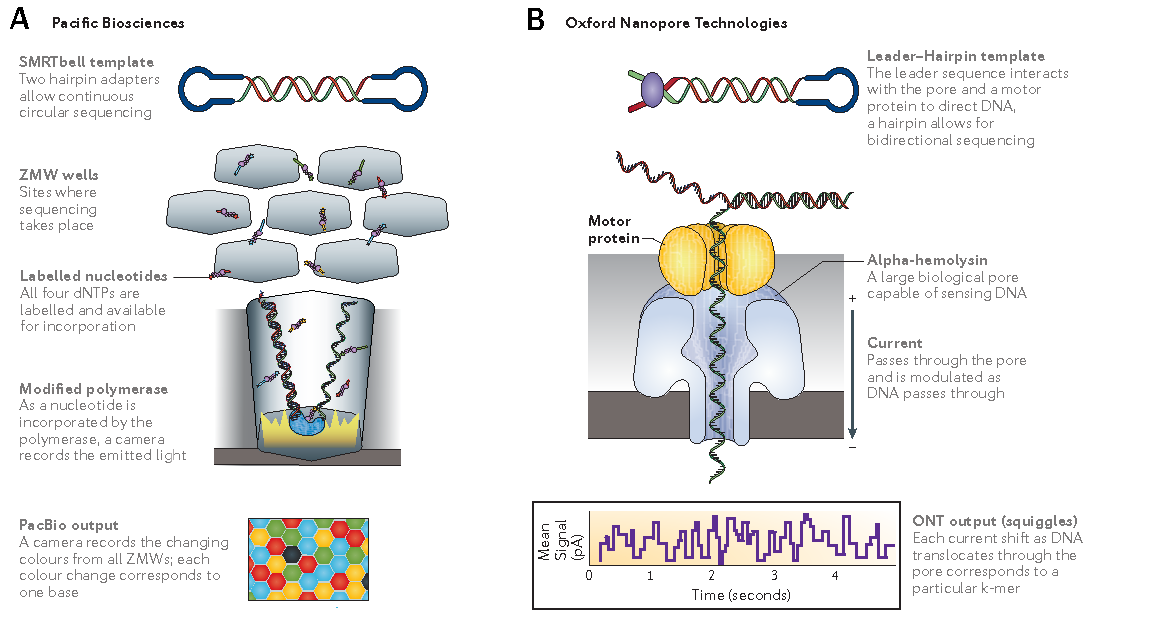
\includegraphics[width=\textwidth]{img/long_seqs.pdf}
    \caption[Fundamentos de la secuenciación de lecturas largas de PacBio y Oxford 
    Nanopore]{Fundamentos de la secuenciación de lecturas largas de PacBio y Oxford 
    Nanopore.(\textbf{A}) Secuenciación SMRT de PacBio: Las plantillas SMRTbell 
    contienen adaptadores en horquilla en ambos extremos que permiten la 
    secuenciación circular continua de ambas hebras de ADN. Estas plantillas se 
    inmovilizan en pocillos ZMW (\textit{zero-mode waveguides}) donde una 
    polimerasa modificada incorpora nucleótidos marcados con fluorescencia. 
    Durante la síntesis, una cámara registra las emisiones de luz 
    correspondientes a cada base incorporada, generando cambios de color que se 
    traducen en la secuencia de bases. (\textbf{B}) Secuenciación por nanoporos 
    de Oxford Nanopore Technologies: La plantilla de ADN contiene una secuencia 
    líder y un adaptador en horquilla que permiten la secuenciación bidireccional. 
    La secuencia líder interactúa con una proteína motora que controla la 
    translocación del ADN a través de un nanoporo biológico (alfa-hemolisina). 
    Al atravesar el poro, el ADN modula la corriente eléctrica de forma 
    específica para cada k-mero (secuencia consecutiva de k nucleótidos, 
    típicamente 5-6 bases). Las señales de salida (\textit{squiggles}) representan 
    estas modulaciones de corriente a lo largo del tiempo, que son posteriormente 
    decodificadas mediante algoritmos de basecalling para obtener la secuencia 
    de bases. Reproducido de \cite{goodwin_coming_2016}.}
    \label{fig:long_seqs}
\end{figure}

\begin{figure}[htbp]
    \centering
    \includegraphics[width=\textwidth]{img/T2T_ref.pdf}
    \caption[Huecos resueltos por el ensamblaje T2T]{Huecos resueltos por el 
    ensamblaje T2T. Cada barra representa la visualización lineal de un 
    cromosoma, con los números cromosómicos indicados a la izquierda. Los 
    segmentos rojos denotan secuencias previamente ausentes que fueron 
    resueltas por el Consorcio T2T en 2022. El cromosoma Y no está incluido, 
    ya que su compleja arquitectura, particularmente sus grandes repeticiones 
    invertidas (IRs) dispuestas en tándem, requirió análisis adicionales y fue 
    publicado de forma independiente en 2023 \cite{rhie_complete_2023}. 
    Adaptado de \cite{zahn_filling_2022}.}
    \label{fig:T2T_ref}
\end{figure}


\begin{figure}[htbp]
    \centering
    \includegraphics[width=\textwidth]{img/ont_pores.png}
    \caption[Mejoras del nanoporo R10 respecto a R9]{El diseño del nanoporo R10 
    introduce mejoras clave respecto a su predecesor R9: una estructura en barril 
    más largo y una arquitectura con doble paso de lectura. Estos cambios
    estructurales permiten una mejor resolución de regiones homopoliméricas como 
    las VNTRs, incrementando significativamente la precisión de consenso de los datos de 
    secuenciación por nanoporos. Reproducido de 
    \cite{oxford_nanopore_technologies_r103_2020}.}
    \label{fig:ont_pores}
\end{figure}


\FloatBarrier


\begingroup
\footnotesize
\begin{longtable}{>{\RaggedRight\arraybackslash}p{3.5cm} >{\RaggedRight\arraybackslash}p{9.25cm} >{\RaggedRight\arraybackslash}p{2cm}}
    \captionsetup{labelfont=bf}
    \caption[Herramientas de software utilizadas en este trabajo]{\RaggedRight Herramientas de software utilizadas en este trabajo.}\vspace{0.30cm}
    \label{tab:software}\\
    
    \toprule
\textbf{Name} & \textbf{Source} & \textbf{Reference} \\ 
\midrule
\endfirsthead

\multicolumn{3}{@{}l}{\RaggedRight \tablename\ \thetable{} -- Continued} \\
\\
\toprule
\textbf{Name} & \textbf{Source} & \textbf{Reference} \\ 
\midrule \\
\endhead \\
\midrule 
\multicolumn{3}{r}{\footnotesize Continued on next page} \\
\endfoot


\bottomrule
\endlastfoot
\\
Positron v2025.10.1-4        & \url{https://github.com/posit-dev/positron}        & --                                    \\
\\
Snakemake v9.13.5            & \url{https://github.com/snakemake/snakemake}       & \cite{koster_snakemakescalable_2012}  \\
\\
Miniforge v25.9.1            & \url{https://github.com/conda-forge/miniforge}     & --                                    \\
\\
VISOR v1.1.2.1               & \url{https://github.com/davidebolo1993/VISOR}      & \cite{bolognini_visor_2020}           \\
\\
minimap2 v2.30               & \url{https://github.com/lh3/minimap2}              & \cite{li_minimap2_2018}               \\          
\\
SAVANA v1.3.6                & \url{https://github.com/cortes-ciriano-lab/savana} & \cite{elrick_savana_2025}             \\
\\
Severus v1.6                 & \url{https://github.com/KolmogorovLab/Severus}     & \cite{keskus_severus_2025}            \\
\\
Sniffles2 v2.7.2             & \url{https://github.com/fritzsedlazeck/Sniffles}   & \cite{smolka_detection_2024}          \\
\\
SVision-Pro v2.5             & \url{https://github.com/sonGBowang125/SVision-pro} & \cite{wang_novo_2024}                 \\
\\
GW v1.2.6                    & \url{https://github.com/kcleal/gw}                 & \cite{cleal_gw_2025}                  \\
\\
UCSC Genome Browser v2025    & \url{https://genome.ucsc.edu/index.html}           & \cite{perez_ucsc_2025}                \\
\\
Wakhan v0.2.0                & \url{https://github.com/KolmogorovLab/Wakhan}      & \cite{ahmad_wakhan_2025}              \\
\\
\end{longtable}
\endgroup

\begin{figure}[htbp]
    \centering
    \includegraphics[width=\textwidth]{img/GW_UI.pdf}
    \caption[Inspección de alineamientos para validación de SVs con GW]{Inspección de alineamientos 
    para validación de SVs con GW. La herramienta se lanza a través de la 
    terminal, solicitando inicialmente la selección del genoma de referencia 
    (\textbf{a}) y abriendo una ventana gráfica vacía. La carga de archivos BAM y 
    VCF que contienen SVs mediante arrastre a la ventana gráfica genera una 
    cuadrícula de imágenes en miniatura correspondientes a los puntos de ruptura 
    indicados en el VCF (\textbf{b}). Al pasar el cursor sobre una imagen se 
    muestran las coordenadas del punto de ruptura en la terminal, mientras que 
    al hacer clic se abre una vista detallada del alineamiento con capacidades 
    de navegación a lo largo del cromosoma (\textbf{c}). El usuario puede
    regresar a la cuadrícula de imágenes y alternar botones Verdadero/Falso en 
    las esquinas inferiores izquierdas para rastrear el estado de validación de 
    las SVs, el cual puede exportarse como una lista para análisis posteriores.}
    \label{fig:GW_UI}
\end{figure}

\newpage

\begingroup
\footnotesize
\begin{longtable}{>{\RaggedRight\arraybackslash}p{3.5cm} >{\RaggedRight\arraybackslash}p{2cm} >{\RaggedRight\arraybackslash}p{2cm} >{\RaggedRight\arraybackslash}p{2cm}}
\captionsetup{labelfont=bf}
\caption[Tamaños de archivos por longitud de lectura]{\RaggedRight Tamaño en gigabytes de archivos de secuenciación de lecturas largas generados con VISOR toolkit a diferentes longitudes de lectura. Los archivos incluyen BAM, sus índices (BAI), y lecturas no alineadas en archivos FASTQ.}\vspace{0.30cm}
\label{tab:file_sizes}\\
\toprule
\textbf{Longitud de lectura} & \textbf{BAM} & \textbf{BAI} & \textbf{FASTQ} \\ 
\midrule
\endfirsthead
\multicolumn{4}{@{}l}{\RaggedRight \tablename\ \thetable{} -- Continuación} \\
\\
\toprule
\textbf{Longitud de lectura} & \textbf{BAM} & \textbf{BAI} & \textbf{FASTQ} \\ 
\midrule \\
\endhead \\
\midrule 
\multicolumn{4}{r}{\footnotesize Continúa en la página siguiente} \\
\endfoot
\bottomrule
\endlastfoot
\\
15000\_normal & 163.88 & 0.0521 & 129.32 \\
\\
15000 & 161.36 & 0.0513 & 127.14 \\
\\
15000 & 161.30 & 0.0513 & 127.15 \\
\\
15000 & 161.22 & 0.0513 & 127.14 \\
\\
30000\_normal & 159.51 & 0.0142 & 127.96 \\
\\
30000 & 156.75 & 0.0140 & 125.79 \\
\\
30000 & 156.79 & 0.0140 & 125.79 \\
\\
30000 & 156.98 & 0.0140 & 125.79 \\
\\
50000\_normal & 157.58 & 0.0091 & 125.85 \\
\\
50000 & 154.63 & 0.0089 & 123.72 \\
\\
50000 & 154.66 & 0.0089 & 123.73 \\
\\
50000 & 154.52 & 0.0089 & 123.73 \\
\\
100000\_normal & 162.33 & 0.0075 & 122.89 \\
\\
100000 & 159.78 & 0.0074 & 120.80 \\
\\
100000 & 159.46 & 0.0074 & 120.80 \\
\\
100000 & 160.12 & 0.0074 & 120.80 \\
\\
\midrule
\textbf{Total} & 2540.86 & 0.3277 & 1998.41 \\
\end{longtable}
\endgroup

\begin{figure}[htbp]
    \centering
    \includegraphics[width=\textwidth]{data/cluster_bmk/calls_data/chr1_del1q21.pdf}
    \caption[Breakpoints de la duplicación en tándem de 1q21 visualizados en GW]{Breakpoints 
    de la duplicación en tándem de 1q21 visualizados en GW. De arriba a abajo: 
    genoma de referencia con barra de escala, posiciones de los breakpoints (marcados con 
    triángulos invertidos), histograma de cobertura de secuenciación (el gris indica 
    concordancia con la referencia), lecturas alineadas, e ideograma del cromosoma 
    (la marca vertical roja señala la región visualizada). Los datos corresponden 
    a la muestra tumoral A con longitud media de lectura de 15 kb.}
    \label{fig:chr1_del1q21}
\end{figure}

\begin{figure}[htbp]
    \centering
    \includegraphics[width=\textwidth]{data/cluster_bmk/calls_data/chr6_inv6q25.1.pdf}
    \caption[Breakpoints de la inversión cromosómica de 6q25.1 visualizados en GW]{Breakpoints 
    de la inversión cromosómica de 6q25.1 visualizados en GW. De arriba a abajo: 
    genoma de referencia con barra de escala, posiciones de los breakpoints (marcados con 
    triángulos invertidos), histograma de cobertura de secuenciación (el gris indica 
    concordancia con la referencia), lecturas alineadas, e ideograma del cromosoma 
    (la marca vertical roja señala la región visualizada). Los datos corresponden 
    a la muestra tumoral A con longitud media de lectura de 15 kb.}
    \label{fig:chr6_inv6q25.1}
\end{figure}

\begin{figure}[htbp]
    \centering
    \includegraphics[width=\textwidth]{data/cluster_bmk/calls_data/chr9_del9p21.3.pdf}
    \caption[Breakpoints de la translocación cromosómica de cortar-pegar en 9p21.3 
    visualizados en GW]{Breakpoints de la translocación cromosómica de cortar-pegar en 9p21.3 
    visualizados en GW. De arriba a abajo: genoma de referencia con barra de escala, posiciones 
    de los breakpoints (marcados con triángulos invertidos), histograma de cobertura 
    de secuenciación (el gris indica concordancia con la referencia), lecturas 
    alineadas, e ideograma del cromosoma (la marca vertical roja señala la región 
    visualizada). Los datos corresponden a la muestra tumoral A con longitud media 
    de lectura de 15 kb.}
    \label{fig:chr9_del9p21.3}
\end{figure}

\begin{sidewaysfigure}
    \centering
    \begin{subfigure}[b]{0.48\textwidth}
        \centering
        \caption*{\textbf{a}}
        \includegraphics[width=\textwidth]{data/cluster_bmk/calls_data/chr11-14_A.pdf}
        \label{fig:chr11-14_A}
    \end{subfigure}
    \hfill
    \begin{subfigure}[b]{0.48\textwidth}
        \centering
        \caption*{\textbf{b}}
        \includegraphics[width=\textwidth]{data/cluster_bmk/calls_data/chr11-14_B.pdf}
        \label{fig:chr11-14_B}
    \end{subfigure}
    
    \begin{subfigure}[b]{0.48\textwidth}
        \centering
        \caption*{\textbf{c}}
        \includegraphics[width=\textwidth]{data/cluster_bmk/calls_data/chr11-14_C.pdf}
        \label{fig:chr11-14_C}
    \end{subfigure}
    \hfill
    \begin{subfigure}[b]{0.48\textwidth}
        \centering
        \caption*{\textbf{d}}
        \includegraphics[width=\textwidth]{data/cluster_bmk/calls_data/chr11-14_D.pdf}
        \label{fig:chr11-14_D}
    \end{subfigure}
    \caption[Breakpoints de la translocación recíproca entre 14q32 y 11q13 
    visualizados en GW]{Breakpoints de la translocación recíproca entre 14q32 y 11q13 
    visualizados en GW. (a) y (b) muestran los breakpoints en el cromosoma 11, 
    (c) y (d) muestran los breakpoints en el cromosoma 14. En cada panel, de arriba 
    a abajo: genoma de referencia con barra de escala, posiciones de los breakpoints 
    (marcados con triángulos invertidos), histograma de cobertura de secuenciación 
    (el gris indica concordancia con la referencia), lecturas alineadas, e ideograma 
    del cromosoma (la marca vertical roja señala la región visualizada). Los datos 
    corresponden a la muestra tumoral A con longitud media de lectura de 15 kb.}
    \label{fig:chr11-14_translocation}
\end{sidewaysfigure}

\begin{figure}[htbp]
    \centering
    \includegraphics[width=\textwidth]{data/cluster_bmk/calls_data/chr17_del17p13.pdf}
    \caption[Breakpoints de la deleción de 17p13 visualizados en GW]{Breakpoints 
    de la deleción de 17p13 visualizados en GW. De arriba a abajo: genoma de 
    referencia con barra de escala, posiciones de los breakpoints (marcados con 
    triángulos invertidos), histograma de cobertura de secuenciación (el gris 
    indica concordancia con la referencia), lecturas alineadas, e ideograma del 
    cromosoma (la marca vertical roja señala la región visualizada). Los datos 
    corresponden a la muestra tumoral A con longitud media de lectura de 15 kb.}
    \label{fig:chr17_del17p13}
\end{figure}

\begin{figure}[htbp]
    \centering
    \includegraphics[width=\textwidth]{img/FISH&CNAs.pdf}
    \caption[Análisis de CNAs de un paciente diagnosticado de mieloma 
    múltiple mediante FISH y secuenciación de lecturas largas]{Análisis de CNAs 
    de un paciente diagnosticado de MM mediante FISH y secuenciación 
    de lecturas largas. (\textbf{A}) Imágenes representativas de FISH realizadas por el 
    personal clínico del Hospital 12 de Octubre que revelan un cariotipo complejo 
    característico de MM: (\textbf{AI}) las sondas específicas de locus (LSI, \textit{Locus-Specific 
    Identifier}) 1q21(\textit{CSF1R})/1p32(\textit{CDKN2C}) detectan ganancia en el número de 
    copias de la región 1p32 (rojo) y número de copias normal de 1q21 (verde); 
    (\textbf{AII}) las sondas XL de tres colores para los genes del cromosoma 13 (\textit{RB1, 
    DLEU, LAMP}) confirman su monosomía; (\textbf{AIII}) sondas LSI 17q22 (\textit{TP53/MPO}) 
    muestran la pérdida de una copia de TP53 (verde) y ganancia de múltiples 
    copias de \textbf{MPO} (rojo). (\textbf{B}) Perfil genómico de número de copias obtenido 
    mediante secuenciación, los recuadros negros indican las regiones cromosómicas 
    correspondientes a las sondas FISH mostradas previamente, mientras que el recuadro 
    morado en línea discontinua señala una disomía uniparental del 4p. Las nubes de 
    puntos rojos y azules representan la profundidad de lectura por bin para los 
    haplotipos HP-1 y HP-2, respectivamente; las líneas horizontales indican números enteros de 
    copias. El paciente presenta alteraciones cromosómicas extensas, incluyendo 
    ganancias (+1q, +3, +4, +15 y +17q) y pérdidas (del 13, del 17p y del 20p), consistentes con el 
    cariotipo complejo típico de MM. Datos provenientes de investigación 
    propia \cite{haertle_multi-omic_2026}}
    \label{fig:FISH_and_CNAs}
\end{figure}


\end{document}